%----------------------------------------------------------------------------------------
%	Part2 - 58Ghz attenuation
%----------------------------------------------------------------------------------------
\newpage

\section{Part2 - 58Ghz attenuation}
From 8 to 14 week I worked for Space technology laboratory supervised by Dr. László Csurgai-Horváth.
Our topic is to research about oxygen and rain attenuation on 58GHz radio signal.

\subsection{Introduction on 58GHz band}
Signal around 60Ghz band has a unique advantage. Around this frequency
signal propagation is effected by oxygen molecule in the air. This phenomenon is 
called oxygen attenuation. Because such phenomenon, signal can not propagate for long distance.
In urban area where high bandwidth communication is required this property can increse
frequency reuse rate which will conserve frequency band resource.

\subsection{Experiment setup}
Two antennas are placed on the roof of building V1 and building E.
An indoor unite was set in the laboratory for data logging.

\paragraph{Geometry}
Geolocation of antennas are measured using GPS coordinate where distance and
elevation angle can be calculated.
GPS coordinates are:
\begin{itemize}
    \item Building V1 antenna: 47.476647, 19.056420, 123.2m
    \item building E antenna: 47.477423, 19.057490, 146.8m
\end{itemize}

From above data we calculated distance $d = 118.0m$ 
and elevation angle $\theta = 11.537^\circ$

\paragraph{Hardware specification}
Testing divices are consist of indoor and outdoor units. Both manufactured by 
Nokia Network. Hardware specification are 
defined in the user manual of these units \cite{metrohopper}
\begin{itemize}
    \item Frequency: 57.725GHz
    \item Polarization: vertical
    \item Antenna gain: 34dB
    \item Transmitter output power: 5dBm
\end{itemize}

\newpage
\subsection{Calculations}
\paragraph{Free space loss}
Free space loss is the loss when signal travels through open space with no
other attenuation. This can be calculated using following equation \cite{openspace}

\begin{equation}
    a_{sz}^{[dB]} = 32.44 + 20log f^{[MHz]}+20log d^{[km]} - G_{TX}^{[dB]} - G_{RX}^{[dB]}
    \label{eq:openspace}
\end{equation}

Where:
\begin{itemize}
    \item $a_{sz}$ is free space loss in dB
    \item $f$ is radio frequency in MHz
    \item $d$ is distance between transmitter and receiver in km 
    \item $G_{TX}$ is transistor antenna gain in dB
    \item $G_{RX}$ is receiver antenna gain in dB
\end{itemize}
\paragraph{Oxygen attenuation}
Oxygen attenuation or Atmospheric attenuation is the effect of signal propagation due to
gas in the atmosphere. The following figure is given in ITU-R P.676 \cite{oxygen} which
demonstrate signal attenuation with different frequency. A peak at around 60GHz is 
clearly visiable which is casued by oxygen molecule in the air.

\begin{figure}[h!]
    \centering
    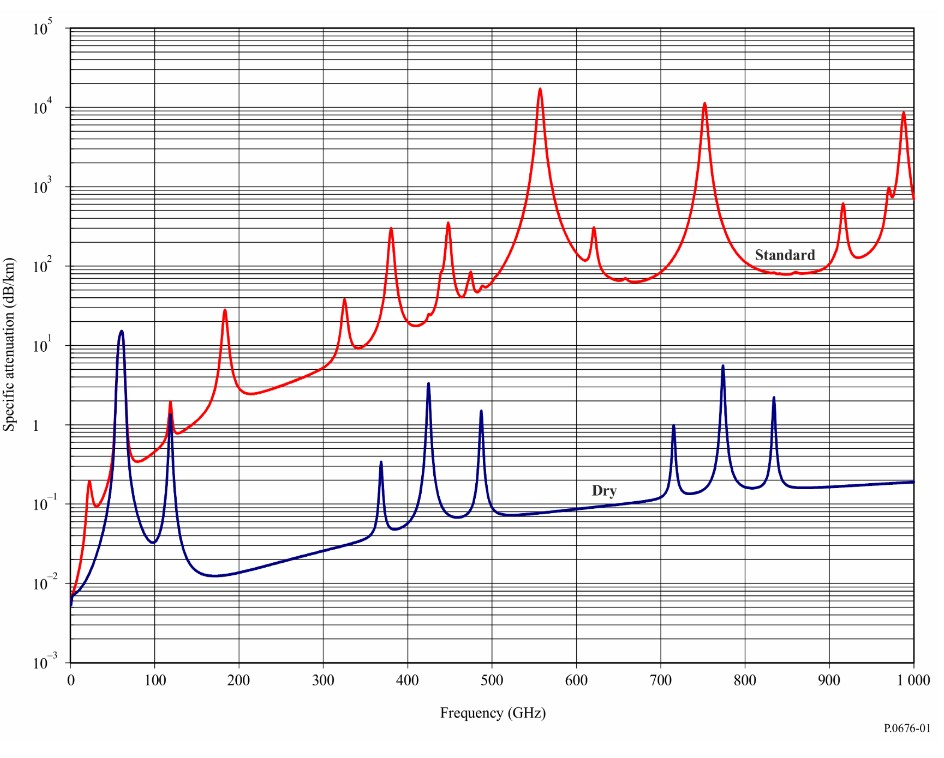
\includegraphics[width=0.9\linewidth]{oxygen.jpg}
    \caption{Atmospheric attenuation}
    \label{fig:Atmospheric attenuation}
\end{figure}

The calculation of oxygen attenuation can be quite complex,
but for the purpose of estimation, the software program Matlab offers
a built-in function \verb|gaspl| that can be used. 

\begin{lstlisting}[language=Matlab]
    L = gaspl(range,freq,T,P,den)
\end{lstlisting}
arguments:
\begin{itemize}
    \item range: Signal path length in multimeters
    \item freq: Signal frequency in Hz
    \item T: Ambient temperature in degrees Celsius
    \item P: Dry air pressure in Pa 
    \item den: Water vapor density or absolute humidity in $g/m^3$
\end{itemize}

\paragraph{Rain attenuation}
Rain attenuation is our main research direction. We want to measure how
rain will effect signal propagation on this particular frequency.
The specific attenuation $\gamma_R$ (dB/km) is obtained from the rain rate $R$ (mm/h)
using the following equation:

\begin{equation}
    \gamma_R = kR^{\alpha}
\end{equation}

Where:
\begin{itemize}
    \item $f$: frequency(GHz)
    \item $k$: either $k_H$ or $k_V$
    \item $\alpha$: either $\alpha_H$ or $\alpha_V$
\end{itemize}

Values for the constants $k$ and $\alpha$ is given in the ITU-R P.838 \cite{rain}

\begin{table}[h]\centering
    \begin{tabular}{|l|l|l|l|l|}
        \cline{1-5}
        Frequency & $k_H$ & $\alpha_H$ & $k_V$ & $\alpha_V$\\
        \cline{1-5}
        58GHz & 0.8226 & 0.7731 & 0.8129 & 0.7552 \\
        \cline{1-5}
    \end{tabular}
    \caption{Frequency-dependent coefficients for estimating specific rain attenuation}
\end{table}

\newpage
\subsection{Measurement result}

We can observe the change of signal level by ploting the signal level over the span of 15 days.

\begin{figure}[h!]
    \centering
    \subfloat[Signal level]{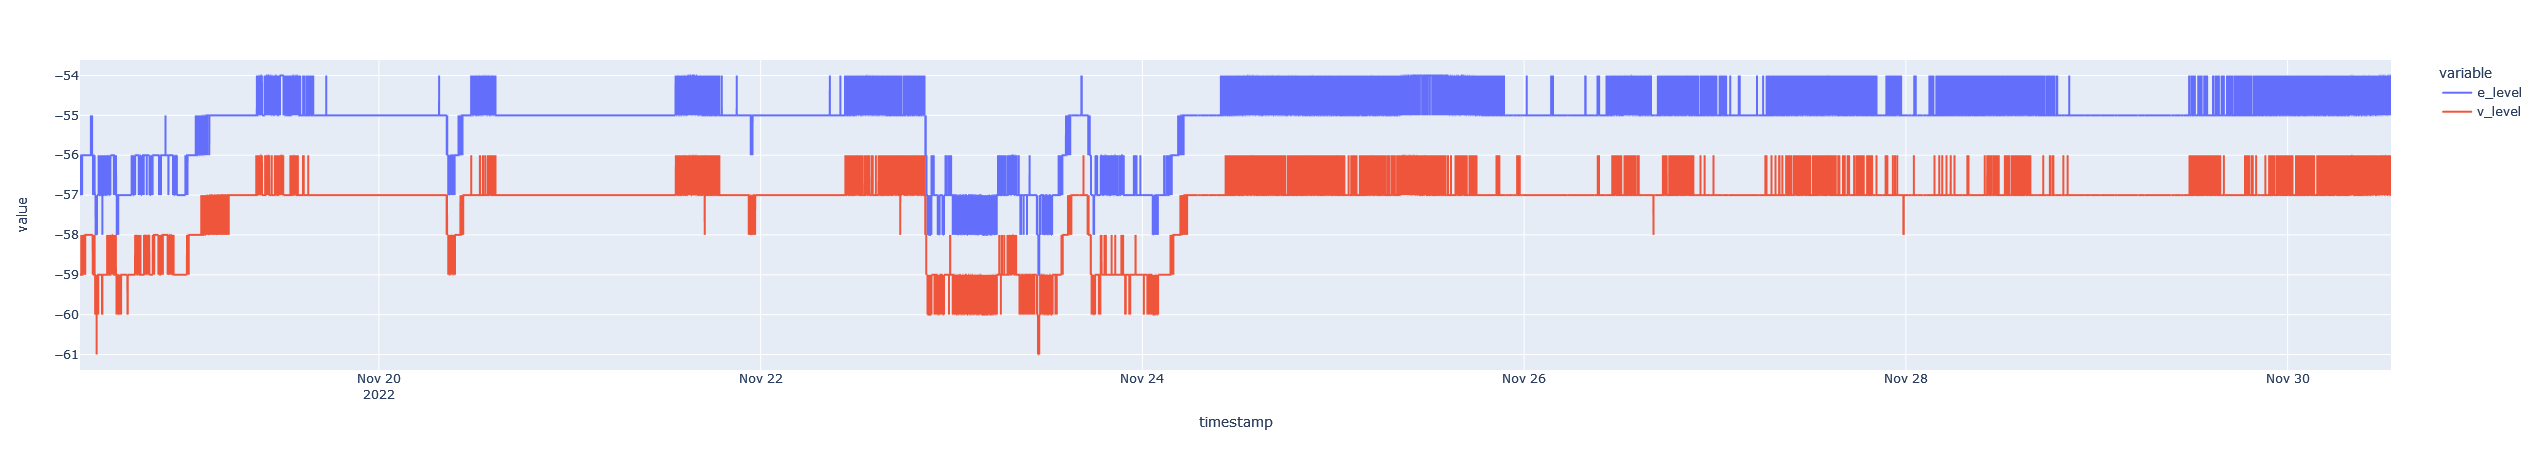
\includegraphics[width=\linewidth]{Figures/signal_nov.png}\centering} \quad
    \subfloat[Weather data]{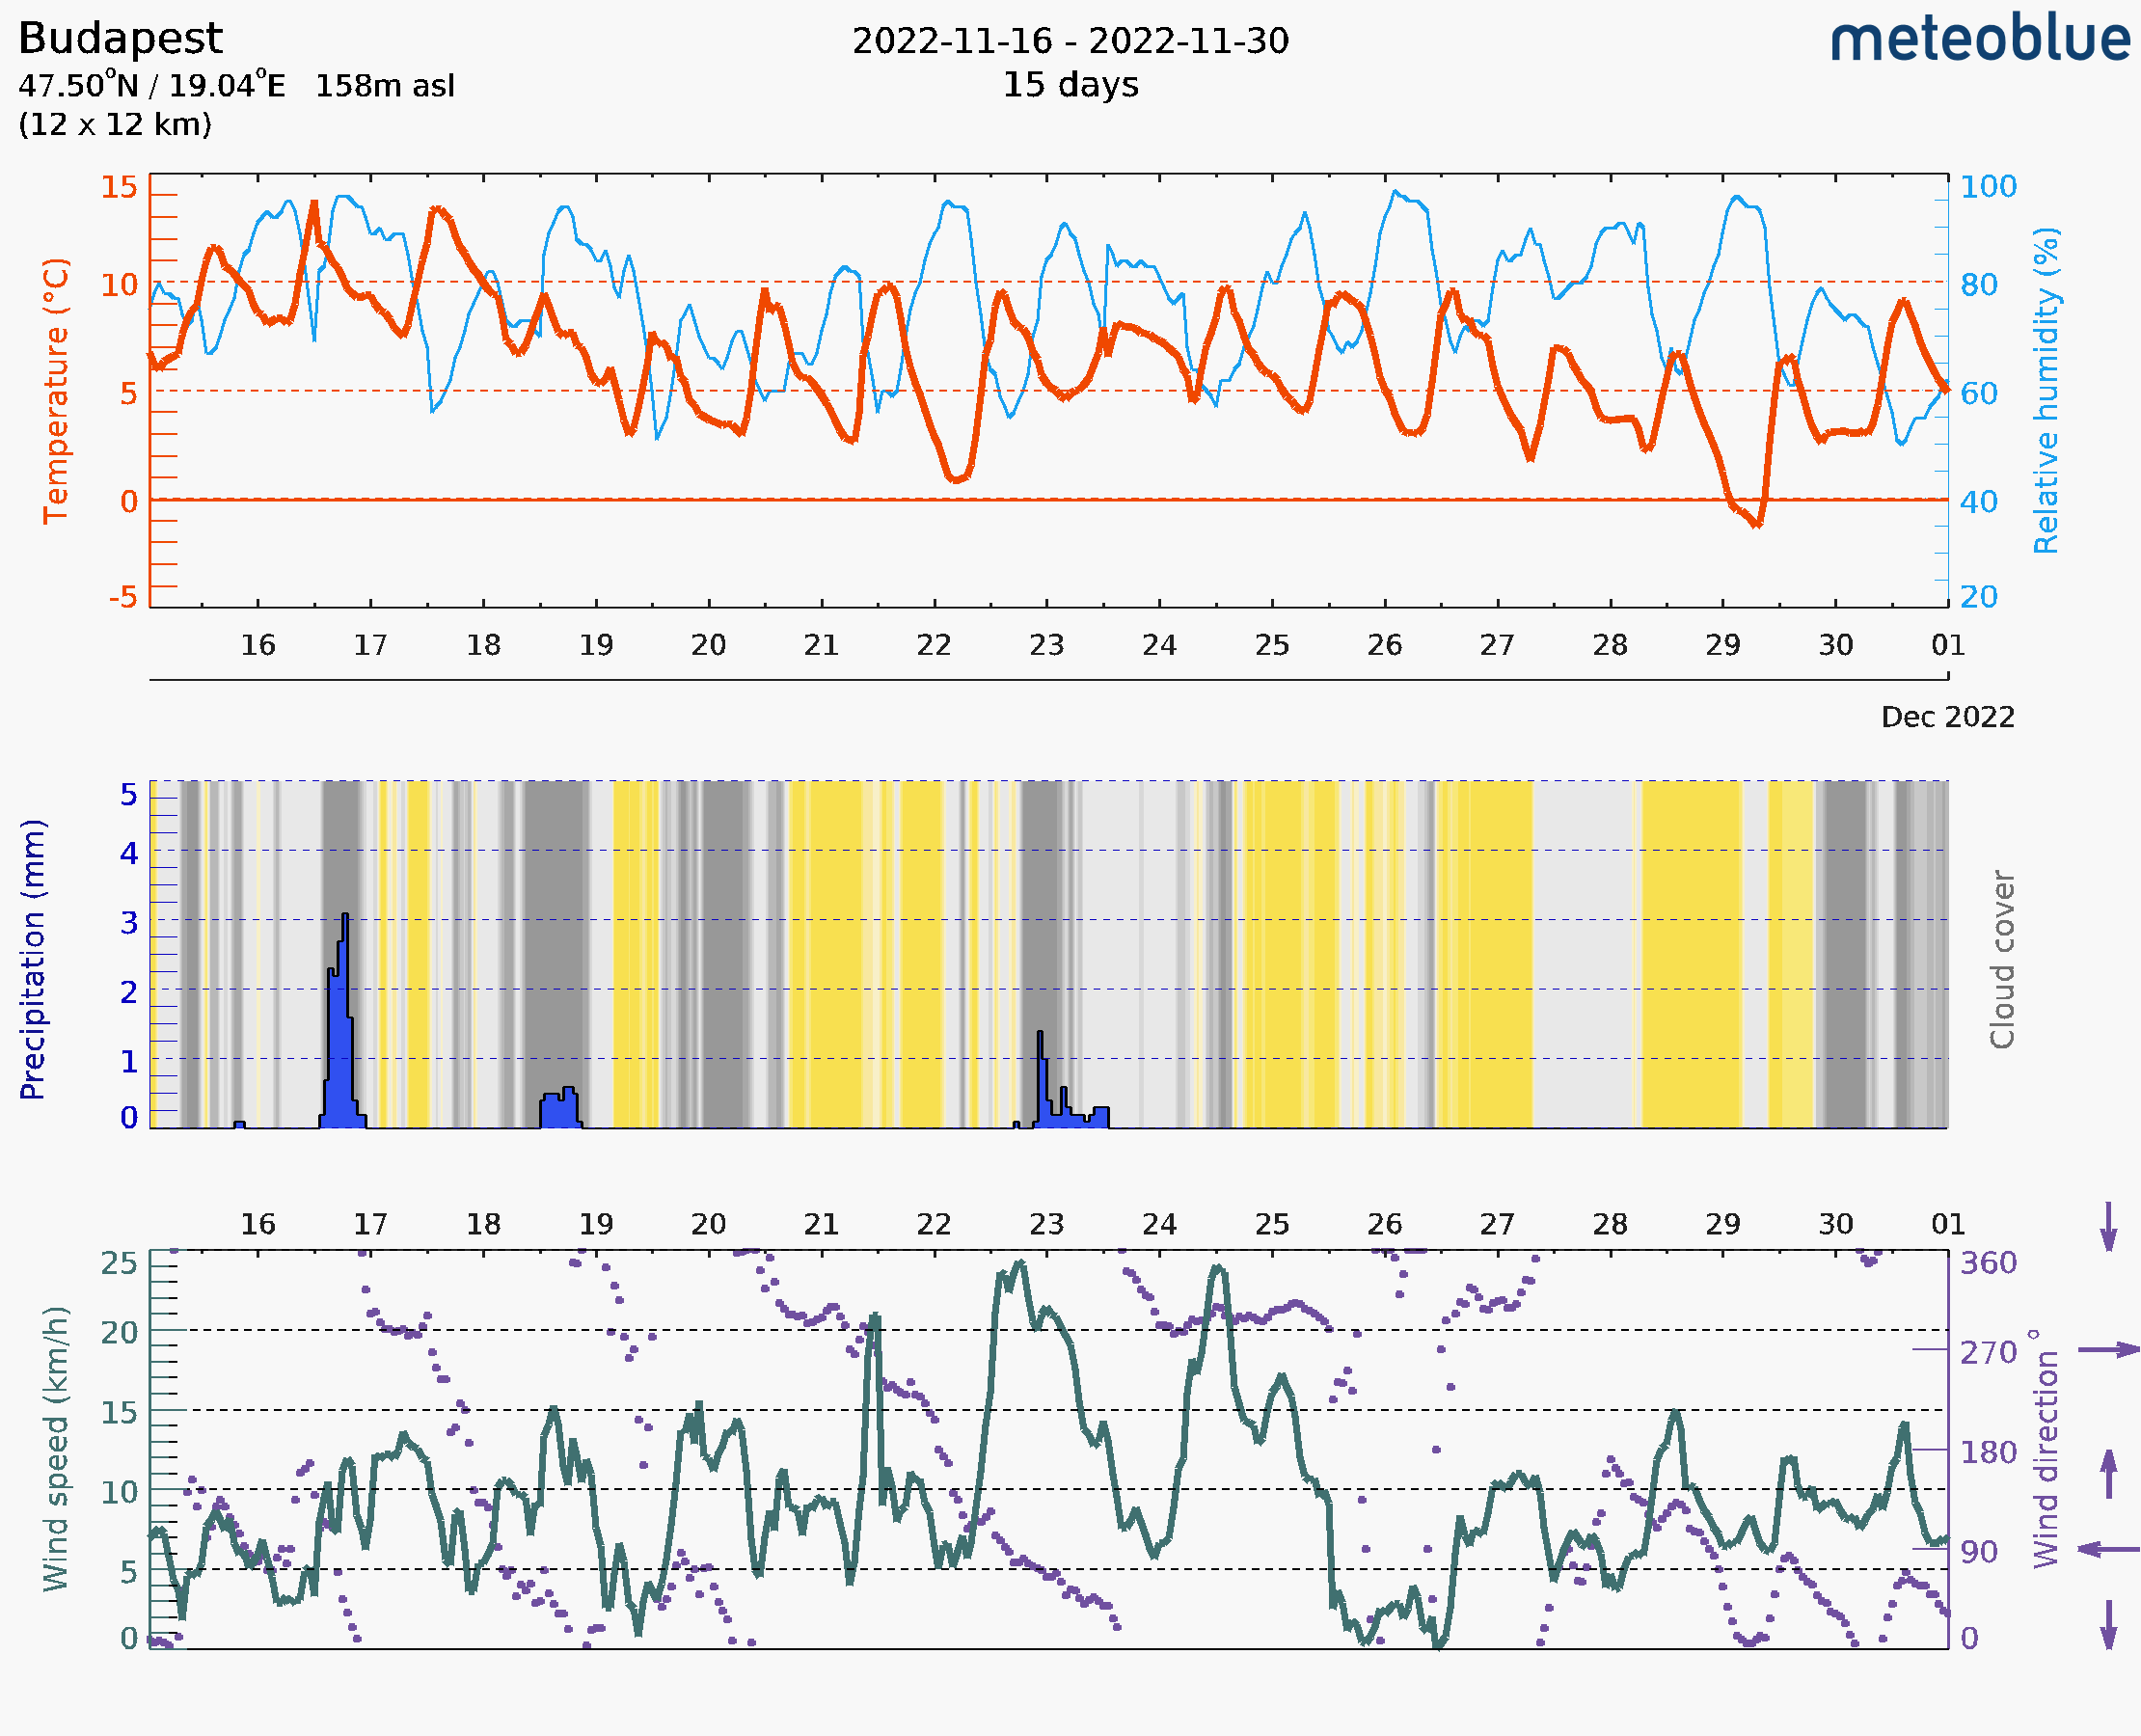
\includegraphics[width=\linewidth]{Figures/weather_history.png}\centering} \quad
 
    \caption{Signal level compared to weather data from 16Nov to 30Nov}
    \label{fig:signal and weather}
  \end{figure}

  Figure 7.a shows the signal level from 16 Nov to 30 Nov. Unfortunately some data are missing because of
  the unreliable data logging software.
  
  Figure 7.b is the historical weather level. \cite{weather}

  We can observe a clear corelation between signal level and precipitation.


\newpage
\subsection{Data processing}
The measurement for this experement happens in a span of several monthes to cover different 
weather condition. Significant amount of data is generated during this process. As a result it is
crucial to save and process the data in a safe and efficient way. I created two program for data processing.
One is running on the data logging computer in the laboratory and the other is running on a cloud server for
data visualisation.

\subsubsection{Data collection}
The measurement data is generated by Nokia HopperManager. A managment software designed to work in pair
with our equipments. The measurement logs are in text file format and is designed to be human readable.
Here is a example of HopperManager log file:

\begin{lstlisting}[
    basicstyle = \tiny
]
    Measurements logged at : 14:40:24 27-10-2022

Unit                            MC Name           Value    Time                 
***************************************************************

OU1A:MetroHopper: Radio InterfacRx level          -57 dBm   14:40:21 27-10-2022
Flexbus 1 far-end: OU1A:MetroHopRx level          -54 dBm   14:40:21 27-10-2022
\end{lstlisting}

I wrote a python program that extract 3 data fields from the log using regex. The signal level of both receiver and a timestamp.
The program then upload these data to a database. This program also support batch uploading. User can sepcify
a directory which contains logfiles and the program will automatically upload all the files.

The following regex pattern is used to match 3 data fields from a logfile.
\begin{lstlisting}[
    basicstyle = \tiny
]
    (?:InterfacRx.+)(-\d{2})(?:\sdBm\s{3})(\d{2}:\d{2}:\d{2}\s\d{2}-\d{2}-\d{4})(?:\n.+\s)(-\d{2})
\end{lstlisting}

\subsubsection{Data visualisation}

I also created a webapp running on Oracle cloud using a lowcode development library called Dash.
User can select a time range on the website and the webapp will fetch the data from database then plot a graph.

\begin{figure}[h!]
    \centering
    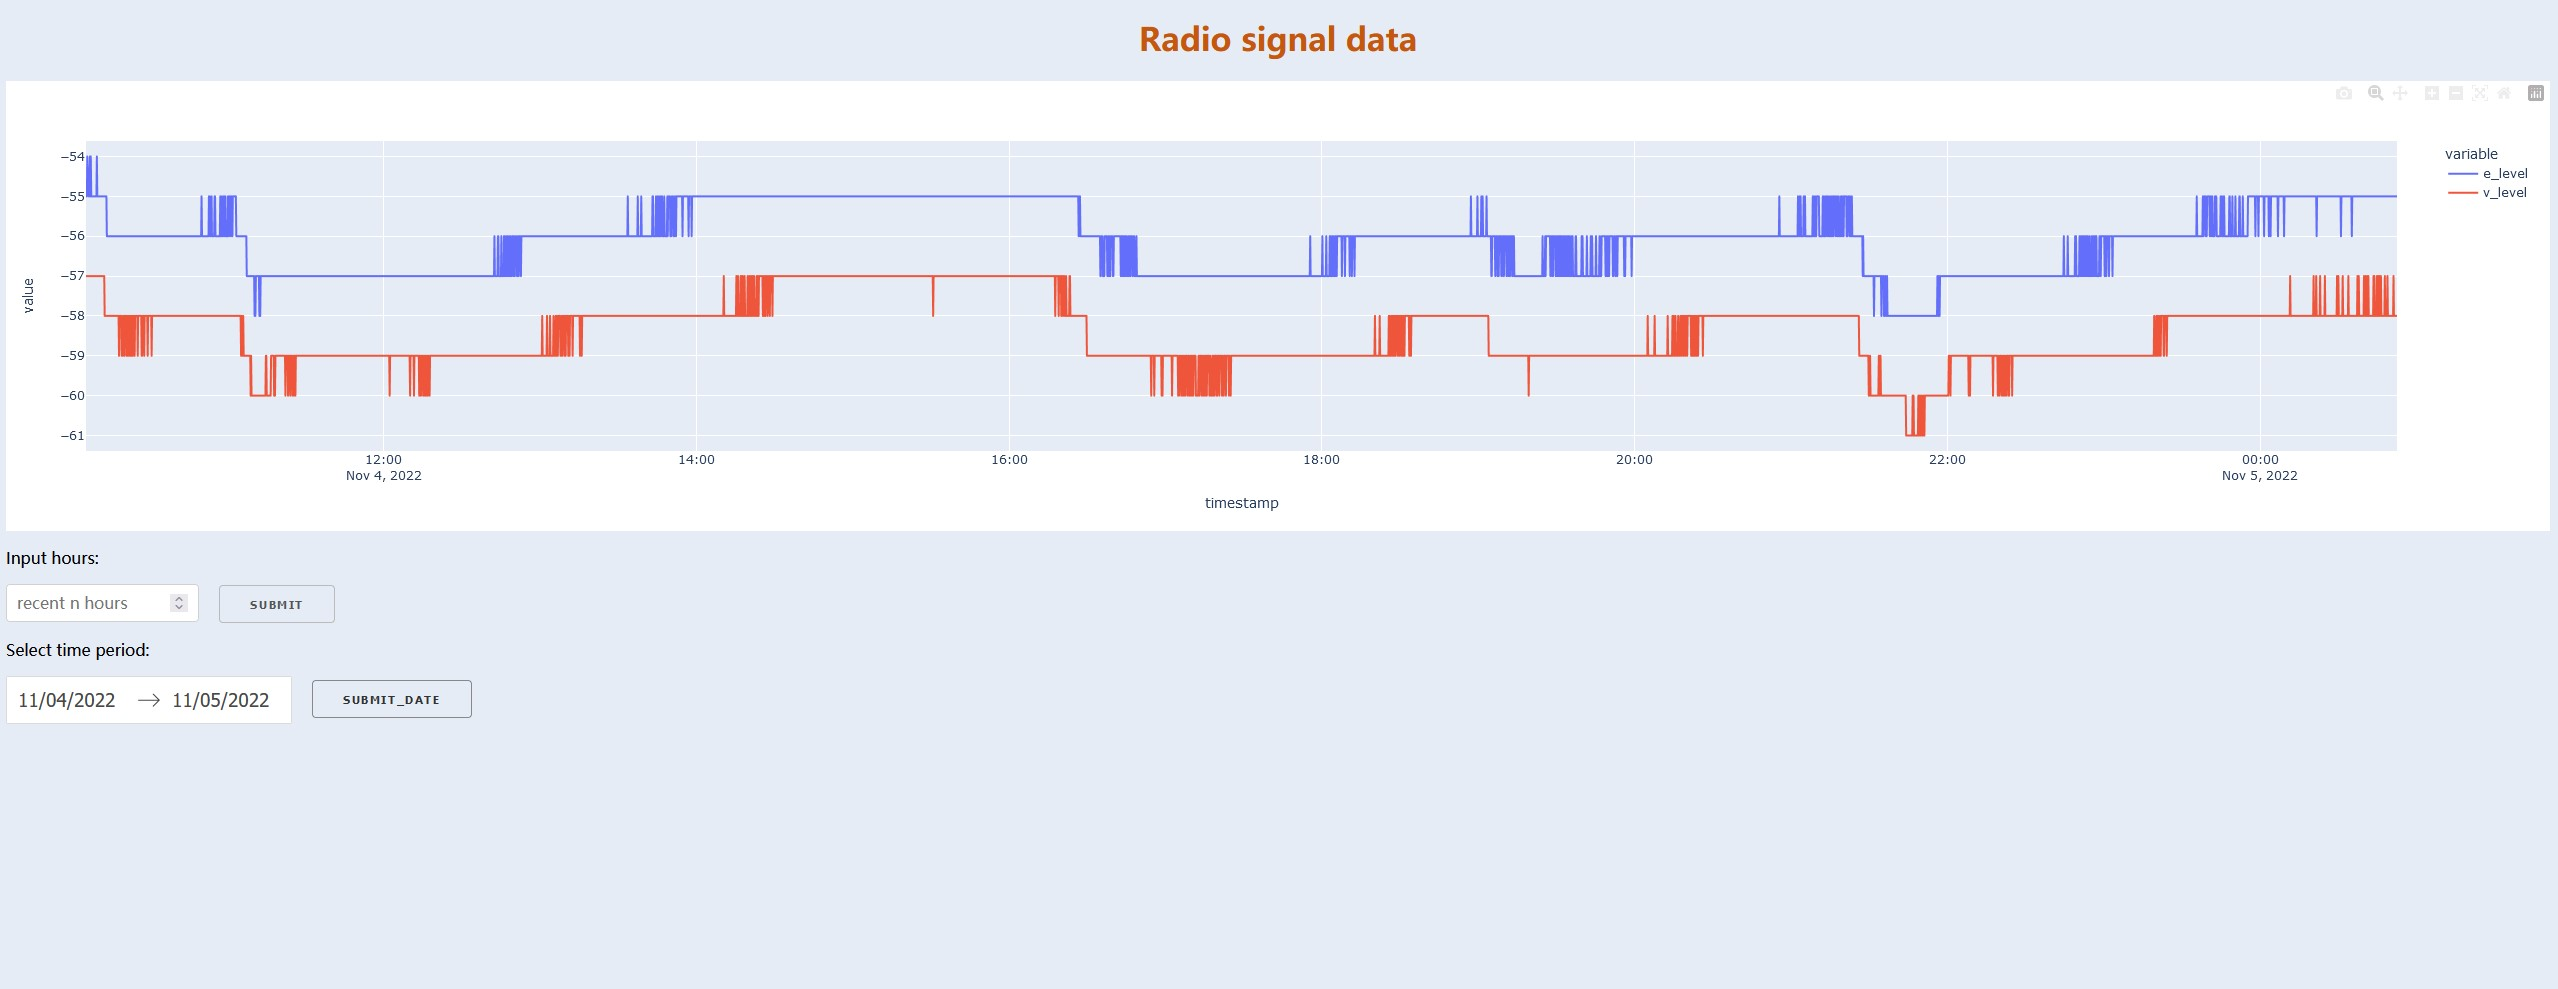
\includegraphics[width=1\linewidth]{dash.jpg}
    \caption{A screenshot of webapp}
    \label{fig:dash}
\end{figure}

The webapp is available at this ip address: \url{http://152.70.177.227:8080/}

\subsubsection{Data storage}

Oracle Cloud Autonomous Database is used to store all the measurement data. This assures that in
an event of a power loss all data will be preserved.

Considering data security reasons, both programs are configured as dedicated database user
who are granted with necessary permition only.

\subsection{Outlook}
\paragraph{Measurement resolution}
The resolution of measurements is only 1dBm and data logging interval is 10 second. Both of these are limitations
of HopperManager. It is possible to increse the resolution to 0.1 dBm and shorten the interval by using the built-in 
scripting tool. But the scripting language is a proprietory standard of Nokia with very limited documentation.

\paragraph{Data collection software}
My original design is to let the program running continuously to achive realtime data uploading.
But since logfiles generated by the script tool is different from current file format it requires
further development to be compatible with newer format.

Also it will be ideal if the data collection software can monitor the system thread of HopperManager
and report automatically in the event of software crash.
The report can be done by using Webhook which can be easily integrated into Microsoft Teams.